\documentclass[margin = 2mm]{standalone}

\usepackage{cascadia-code}
\usepackage[T1]{fontenc}
\usepackage{xcolor}
\usepackage{tikz}

\renewcommand*\familydefault{\ttdefault}

\newcommand{\colorNode}[3]{
	\definecolor{tmpColor}{HTML}{#1}
	\node[below right, background, fill = tmpColor, minimum width = 1.5cm, minimum height = 0.75cm] at (#2, #3) {\MakeUppercase{#1}};
}

\newcommand{\colorNodeInv}[3]{
	\definecolor{tmpColor}{HTML}{#1}
	\node[below right, foreground, fill = tmpColor, minimum width = 1.5cm, minimum height = 0.75cm] at (#2, #3) {\MakeUppercase{#1}};
}

\definecolor{background}{HTML}{1A1416}
\definecolor{foreground}{HTML}{E9DBDF}

\begin{document}
	\pagecolor{background}%
	\color{foreground}%
	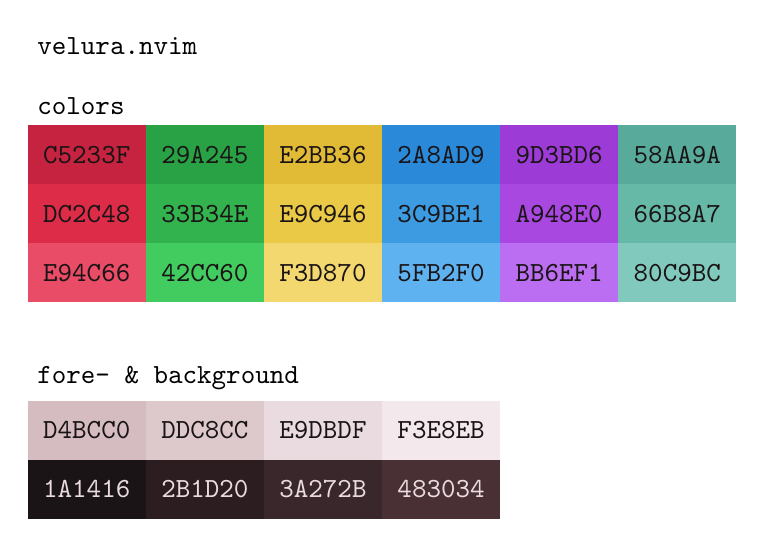
\begin{tikzpicture}%
		\node[right] at (0, 0.5) {\textbf{velura.nvim}};

		\node[above right] at (0, -0.5) {colors};
		% reds
		\colorNode{C5233F}{0.0}{-0.50}
		\colorNode{DC2C48}{0.0}{-1.25}
		\colorNode{E94C66}{0.0}{-2.00}

		% green
		\colorNode{29A245}{1.5}{-0.50}
		\colorNode{33B34E}{1.5}{-1.25}
		\colorNode{42CC60}{1.5}{-2.00}

		% yellows
		\colorNode{E2BB36}{3.0}{-0.50}
		\colorNode{E9C946}{3.0}{-1.25}
		\colorNode{F3D870}{3.0}{-2.00}

		% blues
		\colorNode{2A8AD9}{4.5}{-0.50}
		\colorNode{3C9BE1}{4.5}{-1.25}
		\colorNode{5FB2F0}{4.5}{-2.00}

		% purples
		\colorNode{9D3BD6}{6.0}{-0.50}
		\colorNode{A948E0}{6.0}{-1.25}
		\colorNode{BB6EF1}{6.0}{-2.00}

		% cyans
		\colorNode{58AA9A}{7.5}{-0.50}
		\colorNode{66B8A7}{7.5}{-1.25}
		\colorNode{80C9BC}{7.5}{-2.00}


		\node[above right] at (0, -4.0) {fore- \& background};
		\colorNode{D4BCC0}{0.0}{-4.0}
		\colorNode{DDC8CC}{1.5}{-4.0}
		\colorNode{E9DBDF}{3.0}{-4.0}
		\colorNode{F3E8EB}{4.5}{-4.0}

		\colorNodeInv{1A1416}{0.0}{-4.75}
		\colorNodeInv{2B1D20}{1.5}{-4.75}
		\colorNodeInv{3A272B}{3.0}{-4.75}
		\colorNodeInv{483034}{4.5}{-4.75}
	\end{tikzpicture}%
\end{document}
